The implementation timeline was mostly usecase driven since our team did not have any practical experience with the ROS2 middleware and Gazebo Fortress as a simulator. Because of this we decided early on that we need a way to iterate over different implementations and test sensor feedback from the car platform. In order to get familiar with the ROS2 message formats and the implementation of ROS2 nodes in python using \textit{rclpy} as a dependency we implemented the \textbf{wasd\_control} node. The node is located in the \textit{test\_package} of our ROS2 workspace. The package is utilized as a point in the project where ideas could be implemented and integrated quickly without interrupting the main stack. The control node acts as a keyboard controller for the ackermann steering system and gave us some insights of how the system needs to be updated in order to get a smooth driving behavior. The node implements a state machine that checks for keyboardThis was also the point in the project where we did face the delays that are introduced by the bad network connection available for the project. We experienced control delays from our machine to the vehicle of up to one second which is infeasible for a live feedback loop. This also limited our capabilities of creating visualizations since we had no way of sending them to our monitors since the network bandwidth was so low.



Because of this limitation and the only local availability of the vehicle we moved to implementing the simulation using Gazebo Fortress. In order to work with Gazebo Fortress we had to familiarize ourselves with the concept of modeling for a simulation and in what file format we want to define our models. Ultimately we chose the SDF file format since it is an open source format with relatively new and comprehensive documentation. The URDF and XACRO formats are mainly associated with ROS in the documentation which introduces a barrier, making it harder to work with. These file formats also separate aspects of the same model into different files. This reduces observability of connected components. Having everything in a single file format also reduces complexity since we only had to learn a single new format. In order to implement the vehicle platform and a world around it we heavily utilized the tutorials on the Gazebo documentation \cite{gazebo-documentation}. The first iteration of the vehicle platform was implemented using their \textit{Build your own robot} tutorial and later remodeled once we had a deeper understanding about the file formats and available plugins. At this stage in the development we were able to utilize the examples implemented in the \textit{gazebo\_tutorials} GitHub repository \cite{gazebo-tutorials}. From the repository we learned how to model the Gazebo UI using SDF files and how to implement the transform tree for our vehicle platform in order to have a better transfer to our ROS2 implementation. In the later stages of developing the simulation we focused on getting the data and structure of the messages as close to the real vehicle platform as possible. This was achieved using the ROS2-Gazebo-Bridge \cite{ros-gz-bridge}. With this bridge we could convert the Gazebo-messages to ROS2 messages and forward the topics to ROS2 as well as remap them to the correct paths if necessary. In the end the simulation was close to interchangeable with the implementation of the car platform and we could reuse our complete software stack in the launch files for Gazebo without heavy modifications.

\subsection{Base Control}

Due to the theoretical knowledge we obtained from participating in the lecture about autonomous vehicles and artificial intelligence preceding this project our methodology was to implement the best practices we learned in the lecture. This involves a software architecture comprised of different modules that are responsible for subtasks of the overall driving task. The smallest module we could think of was the task of moving to a point in a given coordinate system. In order to achieve that we experimented with the odometry data coming from the drive controller of the simulation and the vesc module of the F1Tenth system stack. We noticed that the coordinate systems between ROS2 and Gazebo are different and started to implement the required logic using the coordinate system from Gazebo with the plan to implement logic to translate it to ROS2. The coordinate system in Gazebo uses the $y$-direction as forward direction and $-x$ as the direction to the right. In this stage of development the \textbf{MoveToPoint} ROS2 node. This node receives a new target point using \textit{PoseStamped} messages. Once a target point has been received the node checks its current position using a pose it received from some odometry or SLAM (Simoultaneous Localization And Mapping) topic. From the current pose and the target point it calculates a steering angle using the difference in vehicle rotation and target point direction compared to the current vehicle position. This steering angle is of course clipped by the capabilities of the ackermann steering system but recalculated every time the node receives a new vehicle pose estimation, leading to a smooth steering towards the target point. Once a target point is reached, i.e. the distance to the target point is less than a parametrized $\epsilon$, the vehicle stops until it receives a new target point further away.
Figure \ref{fig:move-to-point} visualizes the calculation of the steering angle using the vehicle orientation and the target point. The red circle visualizes the $\epsilon$ distance below which the vehicle will stop approaching the target point.

\begin{figure}[ht]
\vskip 0.2in
\begin{center}
\centerline{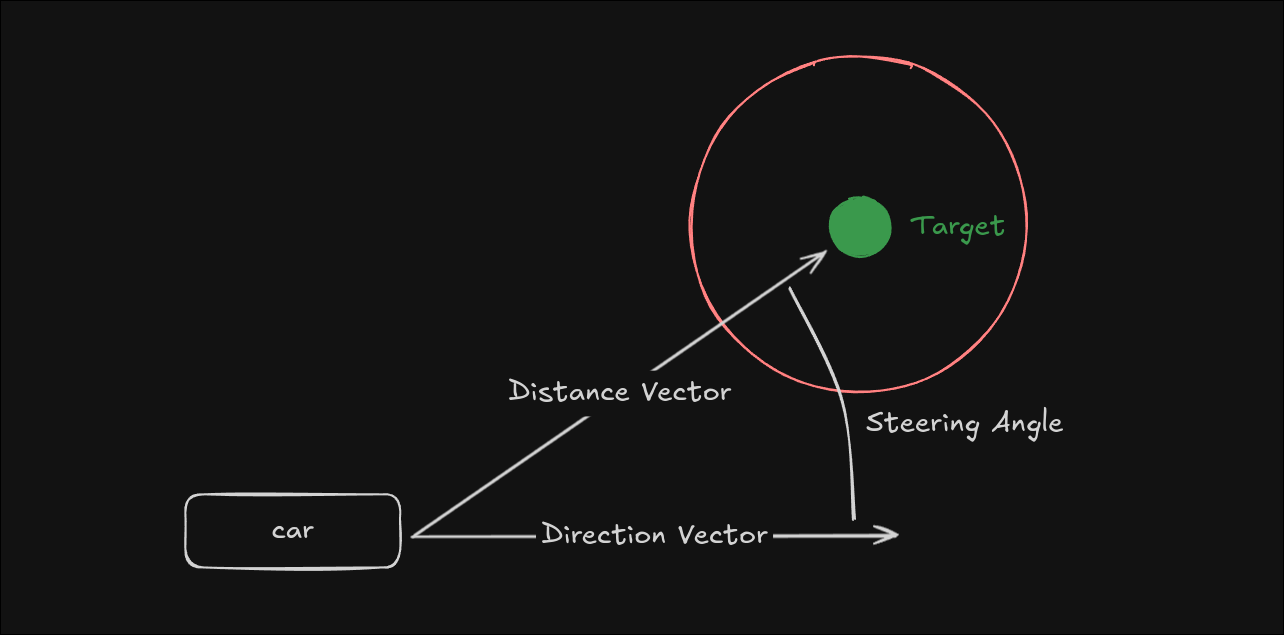
\includegraphics[width=\columnwidth]{move-to-point-vis.png}}
\caption{Schema of the inner workings of the \textit{MoveToPoint} ROS2 node. The figure displays the calculation of the steering angle using vehicle orientation and target point. The red circle marks the $\epsilon$ distance at which the vehicle will stop driving towards the point once inside.}
\label{fig:move-to-point}
\end{center}
\vskip -0.2in
\end{figure}

After iterating over the \textbf{MoveToPoint} node we did notice that the coordinate system of ROS2 was in reality more different than expected which we solved using a custom transform at that time. Due to large drifts in the odometry data of the vehicle in the real world we looked into the next building block for our software stack which was SLAM. SLAM would solve the drifting odometry and provide us with the tools necessary to build a map of the environment that we could enhance with additional information from other sensor systems to create a global plan for driving. Implementing SLAM proved infeasible however since during our experiments we noticed that the transforms from the ROS2 transform tree applied to the sensor data used by the SLAM Toolbox yielded very bad results. The sensor data and map information was drifting a lot. The result was an unusable map and no information about even the immediate proximity of the vehicle. Because of this we tried to create a map without using readily available tools like the SLAM Toolbox which also turned out to be infeasible since the noise of the environment requires robust odometry (roboust meaning it drifts in acceptable margins) and elaborate algorithms that could track objects in the environment over multiple frames of sensor data.

\subsection{Mapping}

Fortunately, after an update of the hardware stack, the transform problems experienced in the context of the SLAM Toolbox were resolved. With stable transforms, we successfully generated accurate maps using LIDAR data processed by the SLAM Toolbox, providing a reliable baseline map for our autonomous navigation tasks.
To further enhance our mapping and navigation capabilities, we integrated semantic information related to cones through a dedicated node, the \textbf{YoloConeDetectionNode}. This node utilizes a YOLO deep-learning model specifically trained on a provided dataset of cone images. The YOLO model facilitates accurate 3D detection of cones while also assigning semantic labels (e.g., the cone colors).
It performs the following key tasks:

\begin{enumerate}
    \item \textbf{2D Cone Detection}: It processes raw RGB images obtained from the Intel RealSense color camera, detecting cones and generating bounding boxes with associated semantic labels indicating the cone type (e.g., the color-based classification).

    \item \textbf{Depth-Based Localization}: To translate these 2D detections into accurate 3D positions relative to the robot, we perform an additional depth-based localization step using the depth information from the RealSense depth sensor, as well as the provided intrinsics and extrinsics from the depth to the color camera. Due to possible misalignments between RGB and depth sensors, direct pixel-to-pixel mapping between color and depth images is not straightforward. Thus, we use an approach analogous to the one used in the Intel RealSense SDK:
    
    \begin{itemize}
        \item \textit{Pixel Correspondence}: For each detected cone, the algorithm identifies the center pixel of its YOLO bounding box in the RGB image. This RGB pixel is then projected onto a corresponding pixel in the depth image through the following procedure:
        
        \begin{enumerate}[label=(\alph*)]
            \item \textbf{Projection to a 3D Line}: The algorithm first takes the RGB pixel coordinates and projects them into two hypothetical 3D points, one at the minimum depth ($depth_{min}$) and one at the maximum depth ($depth_{max}$) limits.
            
            \item \textbf{Image Transformation}: These two 3D points, originally defined in the color image, are transformed into the depth image using pre-calibrated extrinsic parameters.
            
            \item \textbf{Back-Projection to the Depth Image Plane}: The transformed points define a line segment in the depth image plane, representing possible correspondences of the original RGB pixel.
            
            \item \textbf{Optimal Pixel Selection}: The algorithm searches along this line segment in the depth image to find a pixel that, when re-projected into the RGB image, minimizes the distance (error) to the original RGB detection pixel. This step ensures robust and accurate alignment, effectively resolving intrinsic or extrinsic misalignment between sensors.
        \end{enumerate}
        
        \item \textit{Depth Value Extraction and Averaging}: After selecting the optimal depth pixel, the node computes a median depth value from a small pixel patch around it. This averaging further reduces the influence of noise and outliers.
        
    \end{itemize}

    \item \textbf{Transformation using ROS2 TF}: The resulting 3D coordinates are then transformed into the robot's coordinate frame (\texttt{base\_link}) using ROS2's TF2 transformations.
\end{enumerate}

The detected cones will be visualized in RViz via the \textbf{ConeMarkerNode}, which listens to a DetectedConeArray, transforms the cone positions into a target frame, and publishes visual markers to RViz.\\
\newline

The resulting 3D coordinates and their label information are then further used in a \textbf{SemanticMappingNode}, fusing the LIDAR-based map from the SLAM Toolbox with the detected labeled cones to create an occupancy map with semantic information for later use in our planning. The semantic mapping process works as follows:

\begin{enumerate}
    \item \textbf{SLAM Occupancy Grid Processing}:  
    The node subscribes to occupancy grid maps published by the SLAM Toolbox. Upon receiving a new map, it first filters out noise and irrelevant objects based on predefined model assumptions (e.g., maximum object length and minimum object area). This is achieved by identifying connected clusters of occupied grid cells and removing clusters that do not meet these criteria.

    \item \textbf{Cone Detections Integration}:  
    Detected cones from the YOLO-based cone detection node are received. Each cone’s position is transformed from its sensor frame into the global map coordinate frame using ROS2's TF2 transformations, ensuring alignment with the SLAM map and is then stored with a detection timestamp.

    \item \textbf{Semantic Labeling via Cluster Matching}:  
    The filtered occupancy grid is processed to identify connected clusters of occupied cells. Each cluster represents a potential object or obstacle. The algorithm calculates centroids for these clusters, stores them if they are new or matches them against a previously stored cluster, and then compares each centroid’s position against the transformed cones detections. If a cone detection is found within a predefined merge threshold distance, the cluster receives a "hit" corresponding to the cone's semantic label (e.g., cone color).

    Clusters store persistent semantic information by counting the number of hits per label. When assigning semantic labels, each cluster takes on the semantic label with the most hits, providing robust and stable labeling despite potential detection noise or sensor inaccuracies.

    \item \textbf{Semantic Grid Generation}:  
    Finally, a \texttt{SemanticGrid} message is created, containing occupancy information and semantic labels for each cell. Cells in each identified cluster inherit the cluster's dominant semantic label. This semantic map can be directly utilized by downstream exploration and planning modules.

    \item \textbf{Maintenance and Decay}:  
    Cone detections are timestamped and periodically purged based on a decay threshold or if they were already used in the labeling of a cluster. This ensures that outdated or already matched detections do not permanently influence the map’s semantics.

\end{enumerate}

The computational complexity of the semantic mapping process is primarily determined by the following operations:

\begin{itemize}

    \item \textbf{Finding Clusters (Connected-Component Labeling)}:  
    The occupancy grid data (size $n = \text{height} \times \text{width}$) is processed to find connected components using SciPy's \texttt{label} function, which operates in linear time.
    \begin{itemize}
        \item \textbf{Minimum-case:} $\mathcal{O}(n)$
        \item \textbf{Average-case:} $\mathcal{O}(n)$
        \item \textbf{Worst-case:} $\mathcal{O}(n)$
    \end{itemize}

    \item \textbf{Matching Clusters to Stored Clusters}:  
    Each detected cluster (total $k$ clusters) is matched against existing stored clusters (total $s$ clusters) based on centroid distances.
    \begin{itemize}
        \item \textbf{Minimum-case:} $\mathcal{O}(k)$ (if no stored clusters exist, i.e., $s=0$)
        \item \textbf{Average-case:} $\mathcal{O}(k \times s)$
        \item \textbf{Worst-case:} $\mathcal{O}(k \times s)$, which becomes $\mathcal{O}(k^2)$ if $s \approx k$
    \end{itemize}

    \item \textbf{Matching Cones to Clusters}:  
    For each of the $k$ clusters, distances to each of the $m$ cones are computed to assign cone labels to clusters.
    \begin{itemize}
        \item \textbf{Minimum-case:} $\mathcal{O}(k)$ (if $m = 0$)
        \item \textbf{Average-case:} $\mathcal{O}(k \times m)$
        \item \textbf{Worst-case:} $\mathcal{O}(k \times m)$
    \end{itemize}

    \item \textbf{Labeling Clusters}:  
    For each of the $k$ clusters, all grid cells ($n$ total cells) are scanned to determine the cluster cells and assign labels, resulting in complexity $\mathcal{O}(k \times n)$.
    \begin{itemize}
        \item \textbf{Minimum-case:} $\mathcal{O}(n)$ \quad(if there's a single cluster, i.e., $k=1$)
        \item \textbf{Average-case:} $\mathcal{O}(n)$ \quad(if $k$ is small relative to $n$)
        \item \textbf{Worst-case:} $\mathcal{O}(k \times n)$, becoming $\mathcal{O}(n^2)$ in the case where $k \approx n$
    \end{itemize}

\end{itemize}

Combining the above results, the overall computational complexity is summarized as follows:

\begin{itemize}
    \item \textbf{Minimum-case (best-case):} $\mathcal{O}(n + k + k + n) = \mathcal{O}(n + k)\approx \mathcal{O}(n)$

    \item \textbf{Average-case:} $\mathcal{O}(n + k \times s + k \times m + n) \approx \mathcal{O}(n + k \times (s + m))$

    \item \textbf{Worst-case}: $\mathcal{O}(n + k \times s + k \times m + k \times n) \approx \mathcal{O}(k \times (n + s + m))$
\end{itemize}

The \textbf{SemanticGridVisualizerNode} is responsible for visualizing cone clusters detected in a semantic grid using RViz. It processes the semantic occupancy grid, clusters detected cones based on their labels, computes the centroid of each cluster, and publishes visual markers to be displayed in RViz at the location of the centroids.\\


\subsection{Exploration}

Implementing the exploration node after having a semantic map of the immediate environment was very straightforward. Since the semantic map already contains information about cone color and location the only thing that is still missing is the relative position to the vehicle. The SLAM toolbox publishes a \textit{PoseStamped} message containing the position of the vehicle. From this position and the orientation of the vehicle, a projected point is calculated at a parametrizable distance in front of the vehicle. This projection is visualized as the red dot in figure \ref{fig:exploration}. Using this projected position and the location of the cones on the map, the \textbf{Exploration} node calculates the distance to all cones and sorts them in descending order. It then searches for a blue cone to the left by using the sign of the determinant of the matrix comprised of the vehicle position, the projected point and a cone position. If it finds not blue cone to the right it will resort to an unlabeled cone on the map. The same procedure is repeated for the yellow cones to the right. The new target point lies in the center of gravity of the two chosen cones. This target point is then send to the \textit{MoveToPoint} node which then calculates the steering angle and speed to reach it.

\begin{figure}[ht]
\vskip 0.2in
\begin{center}
\centerline{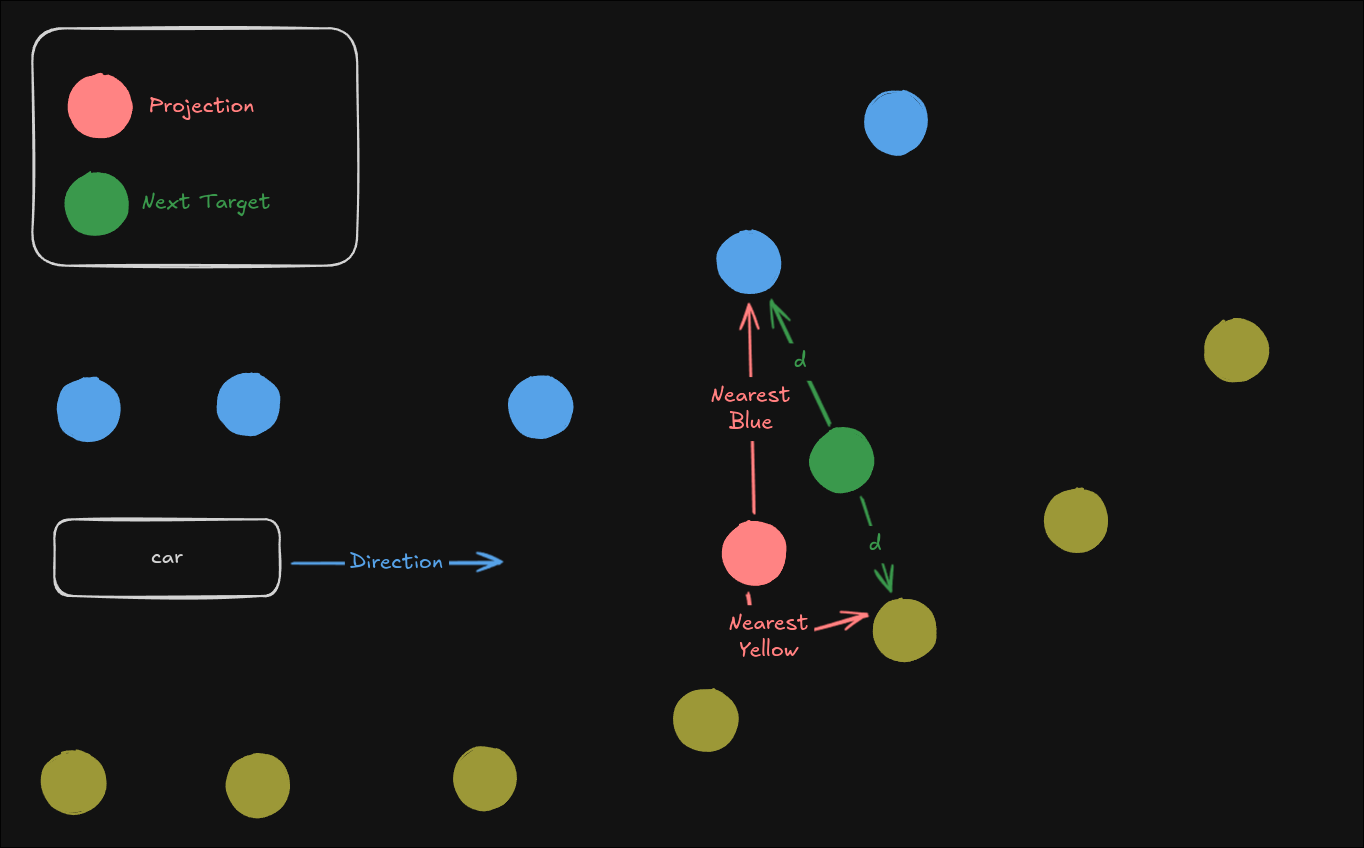
\includegraphics[width=\columnwidth]{exploration.png}}
\caption{Visualization of the calculation of a target point in the textit{Exploration} node. The blue and yellow dots are cones, the red dot is the projected point in front of the vehicle and the green dot the new target point which is send to the \textit{MoveToPoint} node.}
\label{fig:exploration}
\end{center}
\vskip -0.2in
\end{figure}

\subsection{Planning}

The \textbf{GlobalPlanning} node starts out inactive and listens to the vehicle position. Once the vehicle reaches its starting position on the track, marking one finished lap, the node deactivates the \textit{Exploration} node using a service call. Afterwards all the collected vehicle positions are send to the \textit{MoveToPoint} node one as visualized in figure \ref{fig:planning}. Once the vehicle reached the current target point with a certain distance threshold, the next point is published. The node is implemented using a state machine which is using the states \textit{START}, \textit{LEFT\_START}, \textit{FINISHED\_LAP} and \textit{GLOBAL\_PLAN}. during the \textit{START} state the node waits for the vehicle to leave the starting area which is defined as a sphere with parametrizable radius around the starting pose of the vehicle. In the \textit{LEFT\_START} state it will collect the position messages of the vehicle to map out the path driven by the vehicle. Once the vehicle reaches the starting area again the node is switching to the \textit{FINISHED\_LAP} state where it will deactivate the \textit{Exploration} node using a service call. During this state the vehicle will stay still, leaving time to run some optimizations on the collected track information. Afterwards the node switches to the \textit{GLOBAL\_PLAN} state where it will publish the points of the path one by one.


\begin{figure}[ht]
\vskip 0.2in
\begin{center}
\centerline{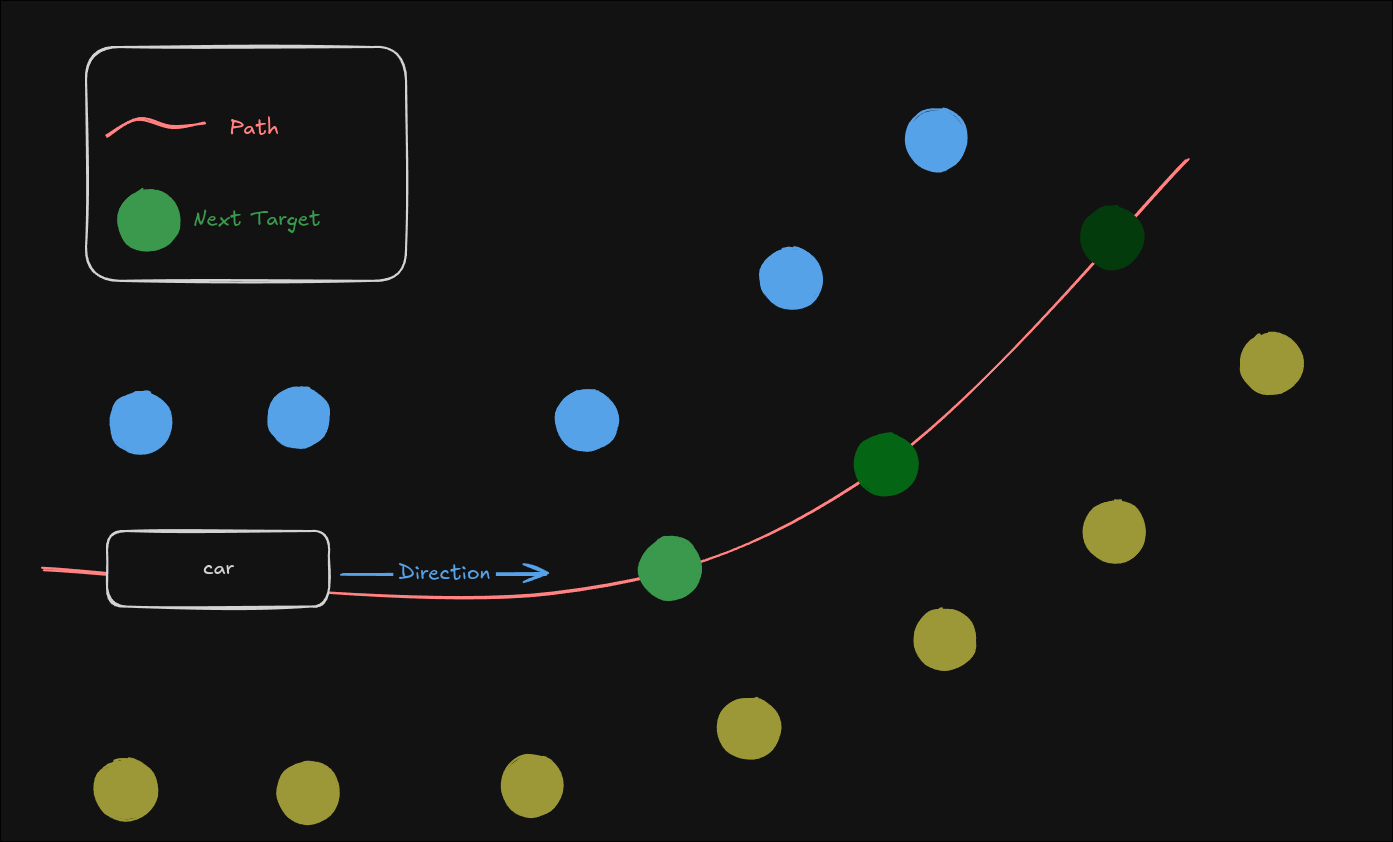
\includegraphics[width=\columnwidth]{planning.png}}
\caption{Visualization of the textit{GlobalPlanning} node. The blue and yellow dots are cones, the green dots are the new target points which are send to the \textit{MoveToPoint} node. After closing in on a point with a certain distance, the next point is published.}
\label{fig:planning}
\end{center}
\vskip -0.2in
\end{figure}
